% !TEX encoding = UTF-8 Unicode
\chapter{基本概念}
\label{chap:chap-2}

\fontsize{12bp}{14.4pt}

\section{代数曲线及其奇点}

\begin{defin}[仿射平面]
\label{defin:affine-plane}
我们称 $\CC^2 = \{(x,y): x,y \in \CC\}$ 为\textbf{仿射平面},
对 $p = (x,y) \in \CC^2$, 称 $x,y$ 为 $p$ 的仿射坐标.
\end{defin}

\begin{defin}[射影平面]
\label{defin:projective-plane}
在拓扑空间 $\CC^3 \setminus \{(0,0,0)\}$ 中引入等价关系 $\sim$:
$(\xi_0,\xi_1,\xi_2) \sim (\xi_0',\xi_1',\xi_2')$ 当且仅当
存在\textit{非零}的 $\lambda \in \CC$ 使得
$\xi_0' = \lambda\xi_0, \xi_1' = \lambda\xi_1, \xi_2' = \lambda\xi_2$.
我们用 $[\xi_0:\xi_1:\xi_2]$ 表示 $(\xi_0,\xi_1,\xi_2)$ 所在的等价类,
称商空间 $(\CC^3\setminus \{(0,0,0)\})/ \sim$ 为\textbf{复射影平面},
记为 $\CP^2$. 对 $p = [\xi_0:\xi_1:\xi_2] \in \CP^2$,
称 $\xi_0, \xi_1, \xi_2$ 为 $p$ 的齐次坐标.
\end{defin}

注意我们有 $\CC^2$ 到 $\CP^2$ 的典范嵌入
$\tau: (x,y) \mapsto [1:x:y]$.
射影平面可以理解成 $\CC^2$ 再添上一条无穷远直线
$L_\infty = \{[0:x:y]: x,y \in \CC\}$.

\begin{defin}[代数曲线]
\label{defin:algebraic-curve}
对 $f(x,y) \in \CC[x,y]$ 以及\textit{齐次}多项式
$F(\xi_0,\xi_1,\xi_2) \in \CC[\xi_0,\xi_1,\xi_2]$,
用 $V(f), V(F)$ 表示它们的零点, 即
\begin{align*}
V(f) &= \{(x,y) \in \CC^2: f(x,y) = 0\},\\
V(F) &= \{[\xi_0:\xi_1:\xi_2] \in \CP^2: F(\xi_0,\xi_1,\xi_2) = 0\}.
\end{align*}
我们称 $V(f), V(F)$ 为 \textbf{仿射, 射影代数曲线}, 记为 $C$,
并称 $f(x,y), F(\xi_0,\xi_1,\xi_2)$ 为 $C$ 的仿射, 齐次方程,
方程的次数称为代数曲线 $C$ 的次数.
若 $C$ 的定义方程 $f(x,y)$ 不可约, 则称 $C$ 为不可约代数曲线.
对一般的 $f(x,y)$, 可以分解为 $f = f_1\cdots f_m$,
此时 $C$ 是一些不可约代数曲线的并 $V(f_1)\cup \cdots \cup V(f_m)$,
每个 $V(f_i)$ 称为 $C$ 的不可约分支.
\end{defin}

若 $C = V(F)$ 由齐次方程 $F(\xi_0,\xi_1,\xi_2)$ 给出,
则我们可以限制在 $\CC^2$ 上看, 得到此时 $C$ 的仿射方程为
\[f(x,y) = F(1,x,y).\]
另一方面, 若 $C = V(f)$ 由仿射方程 $f(x,y)$ 给出, 次数为 $d$,
则它唯一决定了射影代数曲线 $\tilde{C}$,
它的齐次方程为
\[F(\xi_0,\xi_1,\xi_2) = \xi_0^d\cdot f(\xi_1/\xi_0, \xi_2/\xi_0),\]
使得 $\tilde{C}$ 限制在 $\CC^2$ 上就是 $C$.

\begin{exmp}[直线]
\label{exmp:line}
直线就是次数为 $1$ 的代数直线,
由齐次方程
\[A\xi_0 + B\xi_1 + C\xi_2 = 0,\]
$A,B,C \in \CC$ 不同时为 $0$ 决定.
\end{exmp}

\begin{defin}[射影线性变换]
\label{defin:PGL}
称 $\PGL(3, \CC) \defeq \GL_3(\CC)/Z(\GL_3(\CC))$ 为射影线性变换群.
\end{defin}

射影线性变换就相当于 $\CP^2$ 上的坐标变换,
对代数曲线 $C$ 上的一点 $p$,
我们总是能通过适当的坐标变换,
使得 $p$ 具有比较好的齐次坐标.

\begin{exmp}[平移]
\label{exmp:translation}
设 $p = [a:b:c]$ 为代数曲线 $C$ 上一点, 不妨设 $a \ne 0$,
则经过坐标变换
\begin{equation}
\label{eq:translation}
(\xi_0,\xi_1,\xi_2) = (\xi_0',\xi_1',\xi_2')
\begin{pmatrix} 1 &0 &0\\ b &-a &0\\ c &0 &-a \end{pmatrix}
\end{equation}
后, $p$ 的坐标变为 $[a:0:0] = [1:0:0]$.
\end{exmp}

\begin{exmp}[旋转]
\label{exmp:rotation}
设 $p = [1:0:0]$ 为代数曲线 $C$ 上一点,
$L_i, i = 1,2$ 为经过 $p$ 的直线,
则 $L_i$ 的齐次方程为 $B_i\xi_1 + C_i\xi_2 = 0$.
我们可以找到合适的 $\theta$, 通过坐标变换
\begin{equation}
\label{eq:rotation}
(\xi_0,\xi_1,\xi_2) = (\xi_0',\xi_1',\xi_2')
\begin{pmatrix} 1 &0 &0\\ 0 &\cos\theta &\sin\theta\\ 0 &-\sin\theta &\cos\theta\end{pmatrix}
\end{equation}
把直线 $L_1$ 变成直线 $L_2$.
\end{exmp}

现在假设 $p \in \CP^2$ 为一点, $C$ 是一条 $d$ 次不可约代数曲线,
经过适当的坐标变换后, 可以不妨设 $p = [1:0:0]$,
于是限制在 $\CC^2$ 上, $p$ 的仿射坐标为 $(0,0)$.
我们可以把 $C$ 的仿射方程 $f(x,y)$ 写成齐次多项式的和:
\begin{equation}
\label{eq:homo-sum-of-a-polynomial}
f(x,y) = f_0(x,y) + f_1(x,y) + \cdots + f_d(x,y),
\end{equation}
其中 $f_j(x,y) \in \CC[x,y]$ 为 $j$ 次齐次多项式.

\begin{defin}[重数]
\label{defin:multiplicity}
称使得 $f_k(x,y) \ne 0$ 的最小非负整数 $k$ 为点 $p$ 的\textbf{重数}.
\end{defin}

显然 $p \in C$ 当且仅当 $p$ 的重数 $\ge 1$.
注意到因为 $\CC$ 是代数闭域,
每个 $f_j(x,y)$ 都能分解成 $j$ 条直线的乘积, 即
\[f_j(x,y) = (\alpha_1x - \beta_1y)\cdots (\alpha_jx - \beta_jy), \quad \alpha_i,\beta_i \in \CC.\]
直观地看, $p$ 的重数也就是过点 $p$ 有几条 $C$ 的切线.

\begin{defin}[光滑点, 奇点]
\label{defin:smooth-point-and-singularity}
若 $p$ 的重数为 $1$, 则称 $p$ 为 $C$ 的\textbf{光滑点}.
否则, $p$ 的重数为 $k \ge 2$, 此时称 $p$ 为 $C$ 的 \textbf{$k$ 重奇点},
若进一步地 $f_k(x,y)$ 分解成 $k$ 条不同直线的乘积,
则称 $p$ 为\textbf{普通奇点}.
\end{defin}

显然 $p$ 为奇点当且仅当
$\frac{\partial f}{\partial x}(x,y), \frac{\partial f}{\partial y}(x,y), f(x,y)$
在 $p$ 处同时为 $0$.
从射影空间的角度来看,
因为齐次方程和仿射方程的关系为 $f(x,y) = F(1,x,y)$,
所以
\[
\frac{\partial f}{\partial x} = \restriction{\frac{\partial F}{\partial \xi_1}}_{(1,x,y)},
\qquad \frac{\partial f}{\partial y} = \restriction{\frac{\partial F}{\partial \xi_2}}_{(1,x,y)}.
\]
再利用齐次多项式的 Euler 公式
\[\sum_{i=0}^2\xi_i\frac{\partial F(\xi_0,\xi_1,\xi_2)}{\partial \xi_i} = \deg F\cdot F(\xi_0,\xi_1,\xi_2)\]
便知: $p$ 为奇点当且仅当 $\frac{\partial F}{\partial \xi_i}|_p, i = 0,1,2$ 同时为 $0$.

\begin{prop}[直线的 Bezout 定理]
\label{prop:line-bezout}
设 $C$ 是一条 $d$ 次代数曲线, 齐次方程为 $F$.
对任意不是 $C$ 的分支的直线 $L$, 我们有 $\#(C\cap L) = d$.
即 $C$ 与 $L$ 在计算重数的意义下相交于 $d$ 个点.
\end{prop}

\begin{proof}
\footnote{\cite{textbook}, 第一章的定理 8.6}
经过适当的坐标变换后, 不妨设 $L$ 就是直线 $\xi_0 = 0$.
因为 $L$ 不是 $C$ 的分支, 所以 $\xi_0 \ndivides F$.

\begin{claim}
存在适当的 $\lambda \in \CC$, 使得经过坐标变换
\[
\begin{cases}
\xi_0 = \xi_0',\\
\xi_1 = \xi_1' + \lambda\xi_2',\\
\xi_2 = \xi_2',
\end{cases}
\]
后, $F$ 形如
\[F(\xi_0',\xi_1',\xi_2') = (\xi_2')^d + \text{包含 $\xi_2'$ 的低次项}.\]
\end{claim}

事实上, 一开始的 $F$ 形如
\[F(\xi_0,\xi_1,\xi_2) = \sum_{i=0}^da_{i}\xi_1^i\xi_2^{d-i} + \text{包含 $\xi_1, \xi_2$ 的低次项}, \quad a_i \in \CC.\]
因为 $\xi_0 \ndivides F$, 所以 $a_{i}$ 不全为 $0$.
经过坐标变换后, $F$ 形如
\[F(\xi_0',\xi_1',\xi_2') = \paren*{\sum_{i=0}^d a_{i}\lambda^i}(\xi_2')^d + \text{包含 $\xi_2'$ 的低次项}.\]
于是 $a_i$ 不全为 $0$ 便保证了我们希望找到的 $\lambda$ 的存在性.

经过上述坐标变换后, $C$ 与 $L$ 的交点由方程 $F(0,\xi_1,\xi_2) = 0$ 给出.
我们有
\[\#\{F(0,\xi_1,\xi_2) = 0\} = \#\{F(0,\xi_1,\xi_2) = 0: \xi_1 \ne 0\} + \#\{F(0,0,\xi_2) = 0\}.\]
因为 $F(0,0,\xi_2) = (\xi_2)^d$, 所以 $\#\{F(0,0,\xi_2) = 0\} = 0$.
对于 $\#\{F(0,\xi_1,\xi_2) = 0: \xi_1 \ne 0\}$,
相当于求
\[f(x)\defeq F(0,1,x) = x^d + \text{包含 $x$ 的低次项} = 0\]
在 $\CC$ 中有多少个解, 解的个数显然为 $d$.
\end{proof}

\begin{prop}[奇点有限]
\label{prop:finiteness-of-singularity}
一条不可约代数曲线 $C$ 至多有有限多个奇点.
\end{prop}

\begin{proof}
\footnote{\cite{textbook}, 第二章的定理 2.8}
记 $S$ 为代数曲线 $C$ 的所有奇点构成的集合.
将 $C$ 的仿射方程 $f(x,y)$ 视作 $\CC[x][y]$ 中的元素,
则 $\mathcal{D}(x)\defeq \mathrm{disc}(f) \in \CC[x]$,
并且由 $f(x,y)$ 不可约知 $\mathcal{D}(x) \ne 0$.
设 $f_y(x,y) = \frac{\partial f}{\partial y}(x,y) \in \CC[x,y]$,
显然
\[S\cap \CC^2 \subseteq \{(x,y) \in \CC^2: f(x,y) = f_y(x,y) = 0\}.\]
设 $D_x$ 为上式右边的集合在 $x$ 轴的投影,
则由判别式的定义知
$D_x = \{x \in \CC: \mathcal{D}(x) = 0\}$.
显然, $D_x$ 作为一个多项式 $\mathcal{D}(x)$ 的零点集, 是有限集.
其次, 对固定的 $x_0 \in D_x, f(x_0,y) = f_y(x_0,y) = 0$ 作为 $y$ 的多项式
至多只有有限多个根,
这就证明了 $\{(x,y) \in \CC^2: f(x,y) = f_y(x,y) = 0\}$ 是有限集,
从而 $S\cap \CC^2$ 也是有限集.
最后, 因为 $C$ 交无穷远直线 $L_\infty$ 于有限个点(c.f. \cref{prop:line-bezout}),
所以 $S\cap L_\infty$ 也是有限集.
\end{proof}

\begin{exmp}[普通奇点]
\label{exmp:ordinary}
设代数曲线 $C$ 的仿射方程为 $y^2 + x^3 - x^2 = 0$,
则 $p = (0,0)$ 为 $C$ 的二重奇点,
并且因为 $y^2 - x^2 = (y-x)(y+x)$,
所以 $p$ 是二重普通奇点,
两条切线分别为 $y-x=0, y+x=0$.
见 \cref{fig:ordinary} 如下:
\begin{figure}[H]
    \centering
    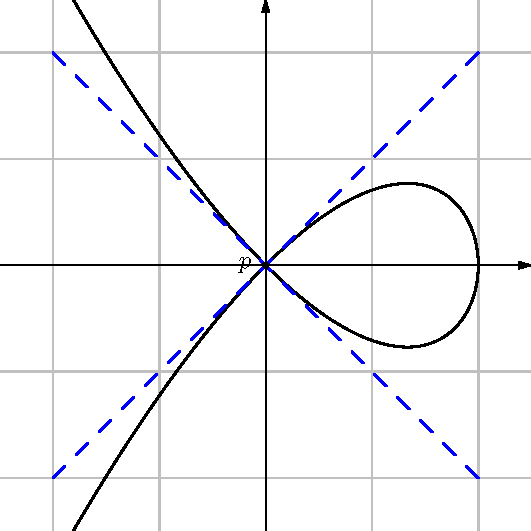
\includegraphics[scale=0.65]{fig-03.pdf}
    \caption{普通奇点, 两条切线}
    \label{fig:ordinary}
\end{figure}
\end{exmp}

\begin{exmp}[非普通奇点]
\label{exmp:non-ordinary}
设代数曲线 $C$ 的仿射方程为 $y^2 - x^3 = 0$,
则 $p = (0,0)$ 为 $C$ 的二重非普通奇点,
两条切线重合(都是 $y = 0$).
见 \cref{fig:non-ordinary} 如下:
\begin{figure}[H]
    \centering
    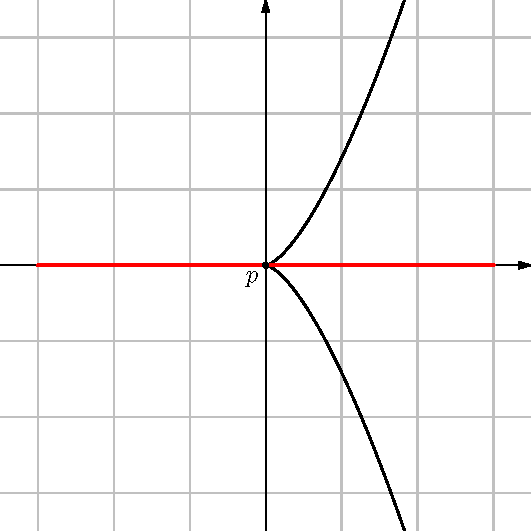
\includegraphics[scale=0.65]{fig-02.pdf}
    \caption{非普通奇点, 切线重合}
    \label{fig:non-ordinary}
\end{figure}
\end{exmp}

\section{Riemann 面及其拓扑}

\begin{defin}[Riemann 面]
\label{defin:2.4}
一个 \textbf{Riemann 面}是指 一个 \textit{连通的 Hausdorff} 空间 $X$,
以及 $X$ 的一个开覆盖 $\{U_\alpha\}$
和一族映射 $z_\alpha: U_\alpha \to \CC$, 称为\textbf{局部坐标系}, 使得
\begin{enumerate}[label=(\arabic*)]
    \ii 每个 $z_\alpha$ 把 $U_\alpha$ 同胚的映到 $\CC$ 的开子集 $z_\alpha(U_\alpha)$;
    \ii 若 $U_\alpha \cap U_\beta \ne \varnothing$, 则\textbf{转移函数}
    \[z_\beta\circ z_\alpha^{-1}: z_\alpha(U_\alpha\cap U_\beta) \to z_\beta(U_\alpha\cap U_\beta)\]
    是双全纯的(i.e., 是一个可逆的全纯函数并且逆也是全纯的).
\end{enumerate}
\end{defin}

和光滑流形类似, Riemann 面就是局部来看都是 $\CC$ 中开集的拓扑空间,
我们可以类似地定义复流形, 而 Riemann 面正是一维复流形.
类似于光滑流形之间的光滑映射, 我们可以定义复流形之间的全纯映射,
并且可以讨论两个复流形是否全纯同构.

\begin{exmp}[Riemann 球面]
\label{exmp:sphere}
射影直线 $\CP^1 = \{[\xi_0:\xi_1]:\xi_0,\xi_1 \in \CC\text{ 不同时为 0}\}$,
扩充复平面 $\ol{\CC} = \CC\cup \{\infty\}$,
以及 $\RR^3$ 中的单位球面 $S$ 是全纯同构的 Riemann 面, 称为 Riemann 球面.
设 $L$ 是 \cref{exmp:line} 中的直线,
注意到对 $[x:y] \in \CP^1$,
存在唯一的 $z$ 使得 $[z:x:y] \in L$,
通过这样的方式, 我们可以把 $\CP^2$ 中的直线都与 $\CP^1$ 等同起来.
\end{exmp}

\begin{exmp}[复射影平面]
\label{exmp:complex-manifold}
$\CP^2$ 是二维复流形. 对任意相同次数的齐次多项式 $F_0, F_1$,
$[\xi_0:\xi_1:\xi_2] \mapsto [F_0(\xi_0,\xi_1,\xi_2),F_1(\xi_0,\xi_1,\xi_2)]$
都是二维复流形 $\CP^2$ 到一维复流形 $\CP^1$ 的全纯映射.
\end{exmp}

\begin{exmp}[复环面]
\label{exmp:torus}
设 $w_1, w_2 \in \CC$ 是 $\RR$-线性无关的, 则它们决定了 $\CC$ 中一个格
\[\Lambda \defeq \{m_1w_1 + m_2w_2: m_1,m_2 \in \ZZ\} \cong \ZZ \oplus \ZZ,\]
格 $\Lambda$ 作为 $\CC$ 的子集有离散拓扑.
在 $\CC$ 中引入等价关系 $\sim$ 使得 $z \sim z' \iff z - z' \in \Lambda$,
得到的商空间 $\CC/\Lambda$ 是 Riemann 面, 称为复环面.
\end{exmp}

因为 $\CC \cong \RR^2$, 并且全纯映射总是光滑的,
所以一个 Riemann 面 $X$ 还能看作一个二维光滑流形,
并且由全纯映射满足 Cauchy-Riemann 方程知,
全纯映射还是保定向的(Jacobi 矩阵行列式 $> 0$),
所以这个二维光滑流形还是可定向的.
如果我们进一步假定 $X$ 还是紧致的,
则由拓扑学中的闭曲面分类定理\footnote{\cite{topo}, 第三章第四节}知,
$X$ 的拓扑被其亏格 $g$ 唯一决定.
注意到此时亏格 $g$ 被 $X$ 的另一个拓扑不变量
欧拉示性数 $\chi(X)$ 唯一决定,
它们的关系是:
\begin{equation}
\label{eq:genus-euler-relation}
\chi(X) = 2 - 2g.
\end{equation}
\cref{exmp:sphere} 和 \cref{exmp:torus} 中的 Riemann 球面和复环面
分别是亏格为 $0, 1$(相应的, 欧拉示性数为 $2, 0$)的 Riemann 面.

\section{Riemann 面之间的映射}
现在假设 $f: X \to Y$ 是 Riemann 面之间的一个非常值全纯映射.

\begin{lem}
\label{lem:surjective}
当 $X$ 是紧致的时候, $f$ 总是满射. 特别的, $Y$ 也是紧致的.
\end{lem}

\begin{proof}
因为紧集的像紧致, 且 $Y$ 作为 Hausdorff 空间, 它的紧致子集必为闭的,
所以 $f(X)$ 在 $Y$ 中闭.
另一方面, 全纯映射总是开映射, 所以 $f(X)$ 在 $Y$ 中开,
由连通性知只能是 $f(X) = Y$.
\end{proof}

\begin{prop}[分歧指标]
\label{prop:ramification-index}
设 $p \in X, q \in Y$ 满足 $f(p) = q$.
则存在 $p,q$ 的局部坐标系 $(U,z), (V,w)$ 使得
$z(p) = w(q) = 0$ 且在这个局部坐标系下 $f$ 形如 $w = f(z) = z^\mu, \mu \in \ZZ_{>0}$.
进一步, 正整数 $\mu$ 与局部坐标系的选取无关,
称为 $f$ 在 $p$ 处的\textbf{分歧指标}, 记为 $\nu_f(p)$,
$p,q$ 分别称为 ramification point 和 branch point.
\end{prop}

\begin{proof}
先任取局部坐标系 $(U',z'), (V,w)$ 使得 $z'(p) = w(q) = 0$,
在这个局部坐标系下 $f$ 形如
\[w = f(z') = (z')^n\cdot h(z'),\]
其中 $n \in \ZZ_{>0}, h(z')$ 是一全纯函数满足 $h(0) \ne 0$.
因为 $h(0) \ne 0$,
所以局部存在全纯函数 $r(z')$ 使得 $r(z')^n = h(z')$(这一点可由广义二项式定理看出),
于是适当的缩小 $U', V$ 后, 我们有 $f(z') = (z'r(z'))^n$.
因为 $r(0) \ne 0, z'r(z')$ 的幂级数展开中 $1$ 次项系数非零,
这意味着存在局部坐标系 $(U,z)$ 使得 $z = z'r(z')$,
在这个局部坐标看, $f$ 形如 $f(z) = z^n$.

设 $(U_1,z_1), (V_1, w_1)$ 是另一组满足条件的局部坐标系,
则存在可逆全纯函数 $\varphi, \psi$ 使得 $z = \varphi(z_1), w_1 = \psi(w)$,
于是 $f$ 在这组新局部坐标系下形如
$w_1 = \psi(w) = \psi(z^n) = \psi(\varphi(z_1)^n)$,
因为 $\varphi, \psi$ 都是可逆的, 所以它们的幂级数展开中一次项系数非零,
由此知 $n$ 是最小的正整数使得
$\psi(\varphi(z_1)^n)$ 幂级数展开中 $n$ 次项系数非零,
这就证明了 $n$ 与局部坐标系的选取无关.
\end{proof}

\Cref{lem:surjective} 告诉我们对任意 $q \in Y$,
存在 $p \in X$ 使得 $f(p) = q$.
\Cref{prop:ramification-index} 告诉我们存在 $p,q$ 的局部坐标系 $U,V$
以及正整数 $\mu = \nu_f(p)$ 使得
$f$ 在这组局部坐标系下形如
\begin{equation}
\label{eq:ramification-local-representation}
w = f(z) = z^\mu, \quad z \in U, w \in V.
\end{equation}
于是: $f^{-1}(0) = 0$,
对任意 $w \in V, w \ne 0, f^{-1}(w)$ 是 $U$ 中 $\mu$ 个不同的点.
换句话说, $f$ 是 $U\setminus \{0\}$ 到 $V\setminus \{0\}$ 的一个 $\mu$ 对 $1$ 的映射:
$f(z) = f(\omega z) = \cdots = f(\omega^{\mu - 1}z)$,
其中 $\omega$ 为 $\mu$ 次单位根.
于是我们有下述推论:

\begin{cor}
\label{cor:preimage-finite}
对任意 $q \in Y, f^{-1}(q)$ 作为 $X$ 的子空间有离散拓扑.
特别的, 当 $X$ 紧致的时候, $f^{-1}(q)$ 为有限集.
\end{cor}

\begin{prop}
\label{prop:ramification-point-finite}
$f$ 在 $U$ 中除 $p$ 外的点处都不分歧,
换句话说, $X$ 中的所有分歧点是离散的.
特别的, 当 $X$ 紧致的时候, 只有有限多个分歧点.
\end{prop}

\begin{proof}
假设对 $p \in U, q \in V, f(p) = q, f$ 在 $p$ 处分歧,
即 $\mu = \nu_f(p) \ge 2$, 则 $f$ 在 $U\setminus \{p\}$ 上是 $\mu$ 对 $1$ 的.
对 $q' \in V\setminus \{q\}$,
设 $p_1,\cdots, p_\mu$ 为 $X$ 中满足 $f(p_1) = \cdots = f(p_\mu) = q'$ 的 $\mu$ 个点.
对每个 $p_i$, 我们考虑 $f$ 在 $p_i$ 处的分歧情况:
存在 $p_i$ 的邻域 $U_i \subseteq U$ 以及 $q'$ 的邻域 $V' \subseteq V$,
使得 $f$ 在 $U_i\setminus \{p_i\}$ 上是 $\nu_f(p_i)$ 对 $1$ 的.
利用 Hausdorff 性质, 我们还可以适当缩小这些 $U_i$ 使得它们两两不交.
现在任取 $\tilde{q} \in V'\setminus \{q'\}$,
则一方面我们有 $\abs{f^{-1}(\tilde{q})\cap U} \ge \sum_{i=1}^\mu \nu_f(p_i)$,
另一方面, 因为 $f$ 在 $U\setminus \{p\}$ 上是 $\mu$ 对 $1$ 的,
所以 $\abs{f^{-1}(\tilde{q})\cap U} = \mu$,
这就推出 $\nu_f(p_i) = 1$.
\end{proof}

\begin{defin}[除子]
\label{defin:divisor}
Riemann 面 $X$ 上的\textbf{除子} $D$ 是一个形式和:
\[D = m_1p_1 + \cdots + m_lp_l,\]
其中 $m_j \in \ZZ, p_j \in X, j = 1,\cdots, l$.
称 $\sum_{j=1}^l m_j$ 为除子 $D$ 的次数, 记为 $\deg D$.
除子之间有自然的加法运算,
$X$ 上所有除子在这个运算下构成一个 Abel 群,
称为 $X$ 的除子群, 记为 $\Div(X)$.
显然 $\deg: \Div(X) \to \ZZ$ 是一个群同态.
\end{defin}

下面总是假设 Riemann 面 $X, Y$ 紧致.

\begin{exmp}[除子的拉回]
\label{exmp:divisor-pullback}
我们可以用全纯映射把 $Y$ 中的除子拉回到 $X$ 中:
设 $q$ 为 $Y$ 中一点, 则 $q$ 也可视作 $Y$ 的一个除子,
定义
\begin{equation}
\label{eq:divisor-pullback}
f^*(q) \defeq \sum_{p \in f^{-1}(q)}\nu_f(p)\cdot p.
\end{equation}
\cref{cor:preimage-finite} 保证了右边实际上是有限和,
所以 $f^*(q) \in \Div(X)$, 再作线性延拓,
我们便有群同态 $f^*: \Div(Y) \to \Div(X)$.
\end{exmp}

\begin{exmp}[分歧除子]
\label{exmp:ramification-divisor}
称
\begin{equation}
\label{eq:ramification-divisor}
R_f \defeq \sum_{p \in X}(v_f(p) - 1)p \in \Div(X)
\end{equation}
为全纯映射 $f$ 的\textbf{分歧除子}.
注意 \cref{prop:ramification-point-finite} 保证了 $R_f$ 是有限和.
\end{exmp}

对任意 $q \in Y$, 定义
\[\Phi(q) = \deg f^*(q) = \sum_{p \in f^{-1}(q)}\nu_f(p).\]

\begin{prop}
$\Phi: Y \to \ZZ$ 是局部常值的.
\end{prop}

\begin{proof}
考虑 $f$ 在所有使得 $f(p) = q$ 的点 $p \in X$ 处的分歧情况.
存在 $q$ 的开邻域 $V$, 还有各 $p$ 点处的开邻域 $U_p$,
使得 $f^{-1}(V) = \bigcup_p U_p$,
且 $f$ 局部地看是 $U_p\setminus \{p\}$ 到 $V\setminus \{q\}$ 的 $\nu_f(p)$ 对 $1$ 映射.
于是, 对所有的 $q' \in V\setminus \{q\}, f^{-1}(q') \cap U_p$ 为 $U_p$ 中 $\nu_f(p)$ 个点,
并且由 \cref{prop:ramification-point-finite} 知这 $\nu_f(p)$ 个点都不是分歧点,
故
\[\sum_{p' \in f^{-1}(q') \cap U_p} \nu_f(p') = \nu_f(p),\]
所以
\[\Phi(q') = \sum_{p' \in f^{-1}(q')}\nu_f(p') = \sum_{p \in f^{-1}(q)}\sum_{p' \in f^{-1}(q') \cap U_p} \nu_f(p') = \sum_{p \in f^{-1}(q)}\nu_f(p) = \Phi(q).\]
\end{proof}

\begin{cor}
$\Phi: Y \to \ZZ$ 是常值映射.
\end{cor}

\begin{proof}
局部常值告诉我们 $\Phi$ 是连续映射,
又因为 $Y$ 连通, 所以 $\Phi$ 必然是常值映射.
\end{proof}

\begin{defin}[全纯映射的次数]
\label{defin:mapping-degree}
任取 $q\in Y$, 称 $\Phi(q)$ 为全纯映射 $f$ 的\textbf{次数}, 记为 $\deg f$.
\end{defin}

\begin{prop}[Riemann-Hurwitz Formula]
\label{prop:Riemann-Hurwitz-Formula}
设 $f:X \to Y$ 是紧 Riemann 面之间的非常值全纯映射,
$R_f$ 为 $f$ 的分歧除子, 则有
\begin{equation}
\label{eq:Riemann-Hurwitz-Formula}
\deg f\cdot \chi(Y) = \chi(X) + \deg R_f.
\end{equation}
\end{prop}

\begin{proof}
见 \cite{textbook} 的第二章的定理 8.5.
\end{proof}
